\documentclass{beamer}

\usepackage[orientation=portrait,size=a1,scale=1.26]{beamerposter}
\usepackage[utf8]{inputenc}
\usepackage[brazil]{babel}
\usepackage{amsmath,amssymb,amsfonts,amsthm}
\usepackage{graphics}
\usepackage{hyperref}
\usepackage{xcolor}
\usepackage[numbers,sort&compress]{natbib}
\usepackage{tikz}

\DeclareMathOperator*{\argmax}{arg\,max}
\usetikzlibrary{positioning,shapes,arrows}
\linespread{1.05}
\definecolor{purple}{HTML}{272686}

\usetheme{Copenhagen}
\setbeamertemplate{headline}{
 \leavevmode
  \begin{columns}[T]
    \begin{column}{.065\linewidth}
        \vspace{1.4cm}
        \hskip1cm
        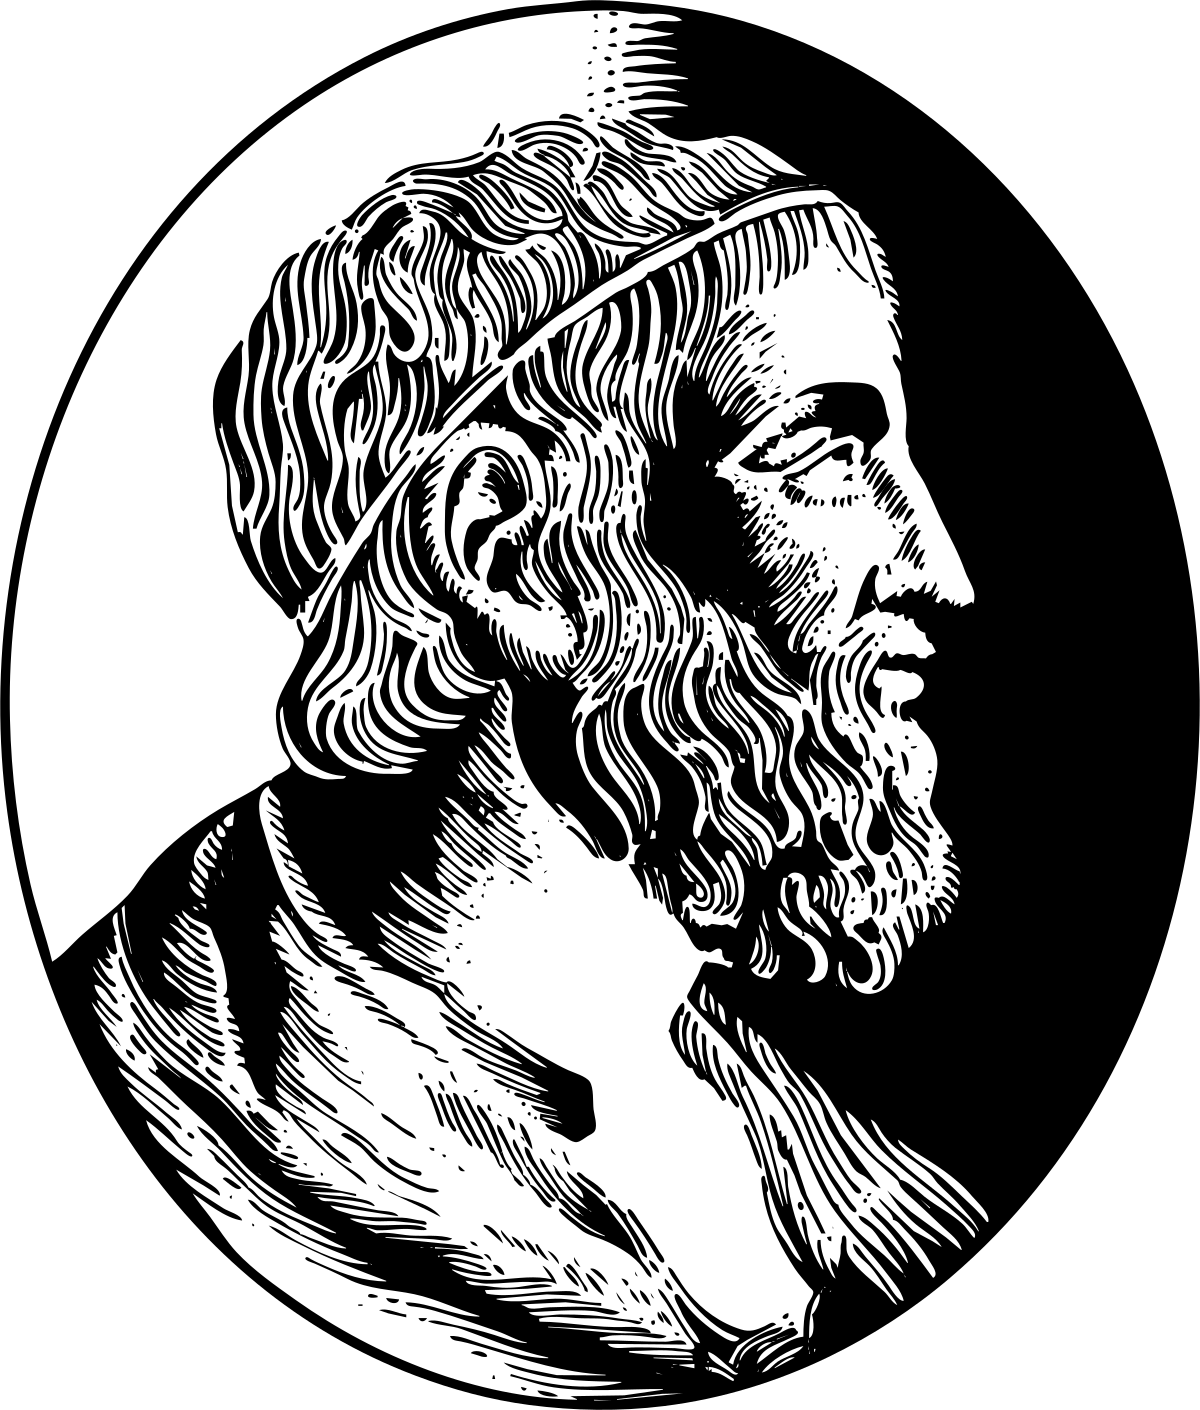
\includegraphics[width=.6\linewidth]{figuras/logo-ime.png}
    \end{column}
        \begin{column}{.87\linewidth}
         \vskip2cm
         \centering
         \usebeamercolor{title in headline}{\inserttitle\\}
         \vspace{1cm}
         \usebeamercolor{author in headline}{\insertauthor\\}
         \vspace{.5cm}
         \usebeamercolor{institute in headline}{\insertinstitute\\}
         \vspace{.5cm}
        \end{column}
    \begin{column}{.065\linewidth}
        \vspace{2.1cm}
        
\includegraphics[width=.88\linewidth]{figuras/logo-usp.pdf}
        \hskip1cm
    \end{column}        
  \end{columns}
  \vspace*{-2.0cm}
}
\setbeamertemplate{footline}{}
\setbeamertemplate{navigation symbols}{}
\setbeamertemplate{caption}[numbered]
\frenchspacing

\title{\color{purple} \Huge \textbf{Funções e tabelas de hash: implementações e aplicações}}
\author{{\Large \textbf{Breno Helfstein Moura}} {\small (Supervisor: José Coelho de Pina Júnior)}}
\institute{\small Trabalho de Formatura Supervisionado do Bacharelado em Ciência da Computação no Instituto de Matemática e Estatística da Universidade de São Paulo (IME-USP)}
\date{Dezembro de 2019}

\begin{document}
\begin{frame}
  
\begin{columns}[t]
\begin{column}{.5\textwidth}
  \begin{block}{Por que estudar \emph{funções e tabelas de hash}?}
    \emph{Funções e tabelas de hash} são amplamente usadas em ciência da computação e engenharia de software. Podemos imaginar funções de hash como uma função que gera uma assinatura digital de um objeto para identificá-lo futuramente. Por sua vez, tabela de hash é uma estrutura de dados que admite operações de inserção, busca e remoção de pares chave-valor. Um dos ingredientes fundamentais é que, funções de hash devem ser parecidas com funções aleatórias, para que exista um número baixo de colisões e as operações em tabelas de hash sejam realizadas eficientemente. 
  \end{block}

  \begin{block}{O que foi feito?}
    Implementações e análises de funções clássicas de hash \cite{TAOCP3}, de diversas de tabelas de hash  e de algumas aplicações utilizando ambas as técnicas.
     Entre as aplicações estudadas temos a verificação de isomorfismo em árvores e, entre as implementações de tabela de hash, temos \textit{Cuckoo Hashing}. 
  \end{block}

  \begin{block}{Como verificar \emph{isomorfismo de árvores}?}
    Durante o filme \textit{Gênio indomável} (1997), Will Hunting (Matt Damon), faxineiro do MIT, resolve um problema deixado em uma lousa da famosa universidade americana. O problema em questão é encontrar todas as árvores homeomorficamente irredutíveis diferentes, de 10 vértices.
    \begin{figure}
      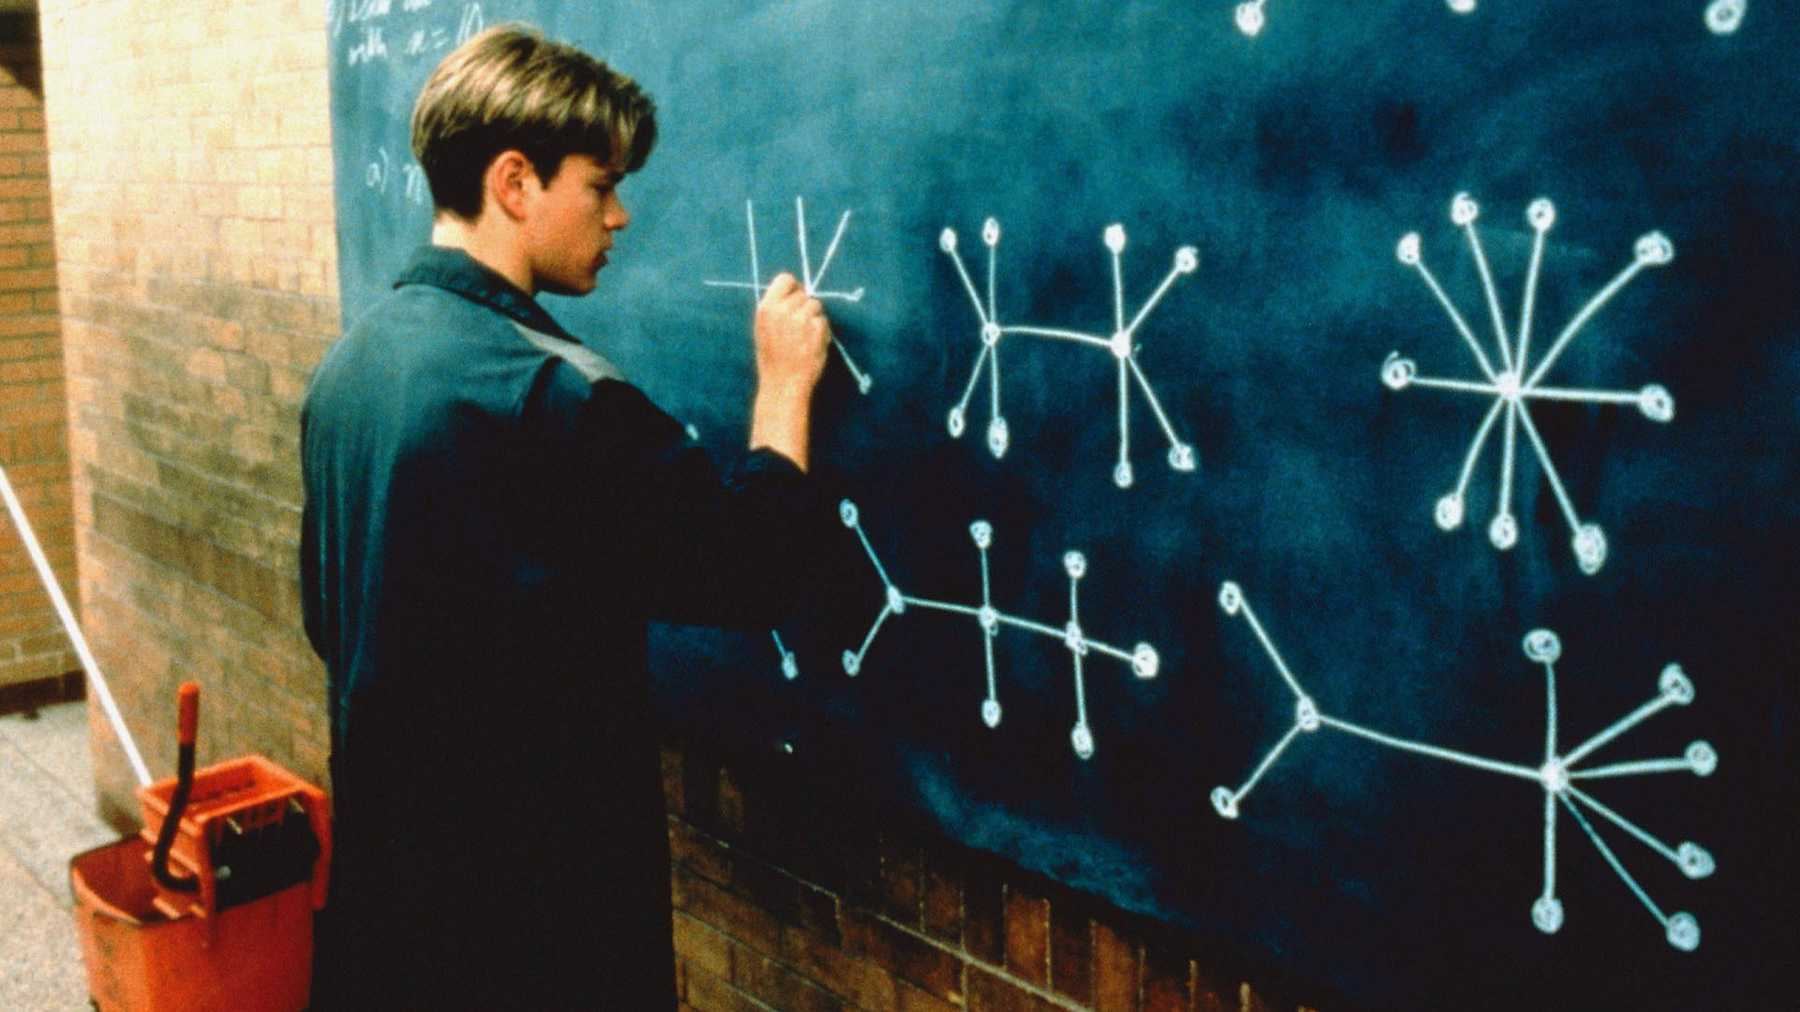
\includegraphics[width=.9\linewidth]{figuras/good-will-hunting.jpg}
      \caption{Cena do filme \textit{Gênio Indomável}}
    \end{figure}

    Mas afinal o que são árvores diferentes? Duas árvores \( T_1 \) e \( T_2 \) são iguais, ou isomorfas, se existe uma bijeção dos vértices de \( T_1 \) para os vértices de \( T_2 \), que preserve as adjacências da árvore. Podemos perceber, que duas árvores são iguais se conseguirmos obter \( T_1 \) a partir de \( T_2 \) renomeando os nós. Logo, duas árvores são diferentes se elas são não isomorfas.
        
    \begin{figure}
      \begin{minipage}{0.3333\textwidth}
        \centering
        \scalebox{1.1}{
          \begin{tikzpicture}
            [scale=.7,auto=left,every node/.style={draw, circle, fill=white, inner sep = 0pt, minimum width = 0.9cm}]
            \node (n1) at (3,8) {1};
            \node (n2) at (1.5,6) {2};
            \node (n3) at (4.5,6) {3};
            \node (n4) at (2.25,4) {4};
            
            \foreach \from/\to in {n1/n2, n1/n3, n2/n4}
            \draw (\from) edge (\to);
          \end{tikzpicture}
        }
        
        (a)
      \end{minipage}\begin{minipage}{0.3333\textwidth}
        \centering
        \scalebox{1.1}{
          \begin{tikzpicture}
            [scale=.7,auto=left,every node/.style={draw, circle, fill=white, inner sep = 0pt, minimum width = 0.9cm}]
            \node (n1) at (3,8) {2};
            \node (n2) at (1.5,6) {1};
            \node (n3) at (4.5,6) {4};
            \node (n4) at (2.25,4) {3};
            
            \foreach \from/\to in {n1/n2, n1/n3, n2/n4}
            \draw (\from) edge (\to);
          \end{tikzpicture}
        }
        
        (b)
      \end{minipage}\begin{minipage}{0.3333\textwidth}
        \centering
        \scalebox{1.1}{
          \begin{tikzpicture}
            [scale=.7,auto=left,every node/.style={draw, circle, fill=white, inner sep = 0pt, minimum width = 0.9cm}]
            \node (n1) at (3,8) {2};
            \node (n2) at (1.5,6) {4};
            \node (n3) at (4.5,6) {1};
            \node (n4) at (5.25,4) {3};

            \foreach \from/\to in {n1/n2, n1/n3, n3/n4}
            \draw (\from) edge (\to);
          \end{tikzpicture}
        }
        
        (c)
      \end{minipage}

      \caption{Três árvores isomorfas}
      \label{fig:isomorfas}
    \end{figure}

    Podemos verificar se as árvores dadas por Will são isomorfas utilizando uma função de hash específica para árvores enraizadas \cite{TreeIsomorphism}. Essa função pode ser calculada de forma recursiva pela seguinte fórmula:

    \[ h(N) = \begin{cases} x_0 ~\text{se N é uma folha da árvore} \\
        \Pi_{i = 1}^{k} (x_d + h(C_i)) mod ~M ~\text{onde} ~C_i ~\text{é um filho de N e d é a altura de N,}
      \end{cases} \]

   onde \( x \) é um vetor de números aleatórios maiores que 0 préfixado. Para calcularmos esse hash precisamos primeiro enraizar as árvores dadas por Will. Podemos enraizar pelo centro ou centroid, pois sabemos que toda árvore tem no máximo dois vértices de centro ou centroid \cite{Centroid}. Abaixo podemos ver duas árvores do filme \textit{Gênio Indomável} enraizadas pelos seus centros:

    \begin{figure}
      \begin{minipage}{0.5\textwidth}
        \centering
        \scalebox{1.1}{
          \begin{tikzpicture}
            [scale=.7,auto=left,every node/.style={draw, circle, fill=white, inner sep = 0pt, minimum width = 0.9cm}]
            \node (n1) at (5,8) {1};
            \node (n2) at (2.0,6) {2};
            \node (n3) at (3.5,6) {3};
            \node (n4) at (5.0,6) {4};
            \node (n5) at (6.5,6) {5};
            \node (n6) at (8.0,6) {6};
            \node (n7) at (3.5,4) {7};
            \node (n8) at (5.0,4) {8};
            \node (n9) at (6.5,4) {9};
            \node (n10) at (8.0,4) {10};
            
            \foreach \from/\to in {n1/n2, n1/n3, n1/n4, n1/n5, n1/n6, n4/n7, n4/n8, n4/n9, n4/n10} 
            \draw (\from) edge (\to);
          \end{tikzpicture}
        }
        
        (d)
      \end{minipage}\begin{minipage}{0.5\textwidth}
        \centering
        \scalebox{1.1}{
          \begin{tikzpicture}
            [scale=.7,auto=left,every node/.style={draw, circle, fill=white, inner sep = 0pt, minimum width = 0.9cm}]
            \node (n1) at (5,8) {1};
            \node (n2) at (2.0,6) {2};
            \node (n3) at (3.5,6) {3};
            \node (n4) at (5.0,6) {4};
            \node (n5) at (6.5,6) {5};
            \node (n6) at (2.0,4) {6};
            \node (n7) at (3.5,4) {7};
            \node (n8) at (5.0,4) {8};
            \node (n9) at (6.5,4) {9};
            \node (n10) at (8.0,4) {10};
            
            \foreach \from/\to in {n1/n2, n1/n3, n1/n4, n1/n5, n2/n6, n2/n7, n5/n8, n5/n9, n5/n10}
            \draw (\from) edge (\to);
          \end{tikzpicture}
        }
        
        (e)
      \end{minipage}
      \caption{Árvores do filme \textit{Gênio indomável}}
      \label{fig:filmtree}
    \end{figure}

    Como ambas árvores possuem altura dois, podemos supor o seguinte vetor \( x \) de tamanho três: \( [13, 1, 9] \). Logo se supormos \( M = 103 \), o valor de hash da árvore (d) seria 19 enquanto o valor de hash da árvore (e) seria 58, e como são diferentes podemos afirmar com certeza que não são isomorfas (Uau! Parte da resposta de Will está correta). Caso fossem iguais poderia ainda ter ocorrido, com baixa probabilidade, uma colisão. Nesse útlimo caso, poderíamos apenas afirmar que as árvores seriam \emph{provavelmente} isomorfas.
  \end{block}
\end{column}

\begin{column}{0.5\textwidth}
  \begin{block}{Como são implementadas tabelas de hash?}
    Tabela de hash é uma estrutura de dados que admite inserção, busca e remoção de pares chave-valor de forma eficiente. Para isso ela se utiliza de funções de hash para indicar as posições na tabela onde um par chave-valor pode ser possivelmente inserido ou encontrado.
    
    % IMAGEM HASH TABLE
    \begin{figure}
      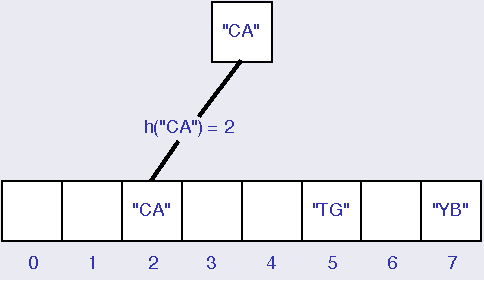
\includegraphics[width=0.6\linewidth]{figuras/hashTable.pdf}
      \caption{Exemplo de uma tabela de hash onde h é a função de hash.}
    \end{figure}

    Contudo, apesar de funções de hash se comportarem idealmente como funções aleatórias, existe uma grande chance de colisão conforme a tabela vai sendo preenchida. Para ilustrar, podemos lembrar do paradoxo do aniversário, que é o fato de que só são necessárias 23 pessoas em uma sala para a chance de duas pessoas terem a mesma data de aniversário ser superior a \(50\%\). Com 57 pessoas a probabilidade é maior que \(99\%\). Podemos perceber que \( \frac{23}{365} = 6.3\%\) e que \( \frac{57}{365} = 15.6\% \). Logo precisamos aprender a lidar com colisões neste tipo de estrutura de dados.
    
    Para lidar com colisões, exitem diversas técnicas, entre elas temos \textit{Linear Probing}, \textit{Quadratic Probing}, \textit{Robin Hood Hashing}, \textit{Chaining Hashing}, \textit{Cuckoo Hashing}, entre outras. Algumas técnicas se utilizam de mais memória que outras, ou possuem mais garantias ou são mais simples de implementar, tendo diversos prós e contras para cada uma das implementações. \textit{Chaining Hashing} por exemplo, é fácil de ser especificado e possui operações muito bem definidas, o que faz dela a implementação preferida para tabelas de hash padrão de linguagens de programação como C++, Java, Golang, C\# e Scala. 
    
    % Imagem Chaining    
    \begin{figure}
      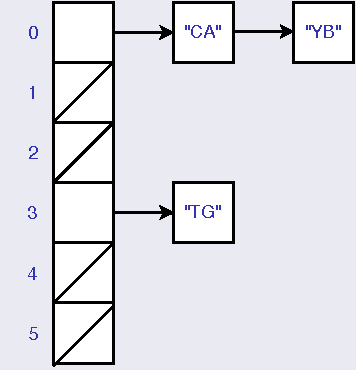
\includegraphics[width=0.35\linewidth]{figuras/chainingHashing.pdf}
      \caption{Ilustração de uma tabela de hashing implementada com chaining hashing}
    \end{figure}

    
  \end{block}

  \begin{block}{Cuckoo Hashing}
    \textit{Cuckoo Hashing} é uma das implementações mais exóticas de tabela de hash, contudo é uma implementação muito interessante, pois possui tempo de busca e remoção constante no pior caso, fato que não é verdade para a maioria das outras implementações \cite{CuckooHashing}.
    Essa implementação de tabela de hash utiliza dois ou mais vetores e duas ou mais funções de hash, e quando existe uma colisão durante a inserção ela move pares chave-valor de um vetor para o outro. O nome Cuckoo vem do passarinho de mesmo nome, que é conhecido por depositar seus ovos em ninhos de outros passarinhos, muitas vezes empurrando os ovos que ali estavam para fora.
    Para mover os pares chave-valor de um vetor para o outro, o algoritmo primeiro insere o par que já estava tentando inserir na posição colidida e então tenta inserir o par que foi removido em outro vetor. Para a busca e remoção basta olhar em todos os vetores na posição para o qual a função de hash indica. Vale mencionar que a maioria das implementações de \textit{Cuckoo Hashing} se utiliza de dois vetores.
    
    % IMAGEM CUCKOO
    \begin{figure}
      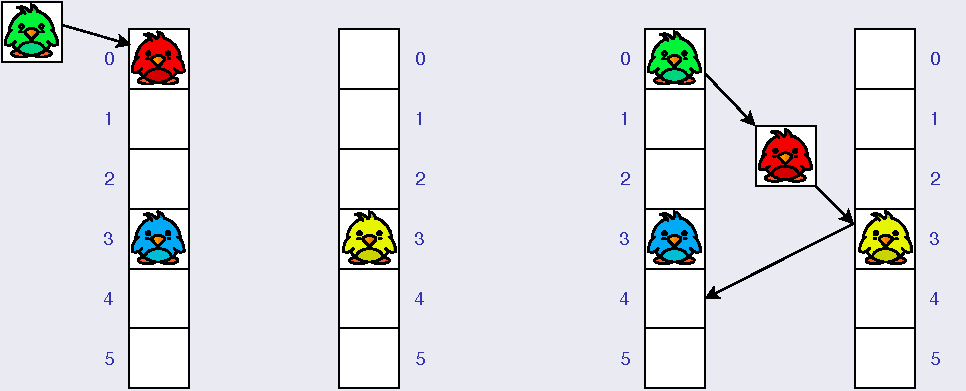
\includegraphics[width=0.75\linewidth]{figuras/cuckooHashingColored.pdf}
      \caption{Ilustração da inserção do cuckoo hashing}
    \end{figure}

    
  \end{block}

  \begin{block}{Mais informações}
    Este pôster, a monografia e os códigos desenvolvidos estão disponíveis em: \url{https://github.com/breno-helf/TCC}
  \end{block}

  \begin{block}{Bibliografia}
    {\scriptsize
    \bibliographystyle{unsrt}
    \bibliography{bibliografia}
    }
  \end{block}
\end{column}
\end{columns}
\end{frame}
\end{document}
